%\documentclass[handout]{beamer}
\documentclass{BeamerTemplate}


\newcounter{sauvegardeenumi}
\newcommand{\asuivre}{\setcounter{sauvegardeenumi}{\theenumi}}
\newcommand{\suite}{\setcounter{enumi}{\thesauvegardeenumi}}


%\usepackage[latin1]{inputenc}  %modifies preambule

\title{La statistique : les grandes idées}
\date{}


\begin{document}

\begin{frame}

\titlepage

\end{frame}

%-------------------------------------------------------------------------------------------------------------------------------------


\begin{frame}{La statistique}

\underline{Objectif de la statistique}: Apprendre sur le monde qui nous\\
\hspace{4.3cm} entoure à partir de données. 

\vspace{0.1in}
\begin{center}
\textit{Statistics : The Art and Science of Learning from Data}
\end{center}


\vspace{0.3in}

\pause

Pourquoi doit-on avoir recours au \alert{raisonnement statistique} en plus du \alert{raisonnement mathématique}?  

\pause
\begin{center}
\textbf{Pour tenir compte de la VARIABILITÉ!}
\end{center}

\end{frame}


\begin{frame}{Variabilité et raisonnement statistique}

Anne-Sophie Charest est-elle plus grande que Mathieu Champigny? \\
\alert{$\implies$ Raisonnement mathématique\\
\hspace{1cm} (comparer deux nombres)}


\pause

\vspace{0.3in}
On mesure tous les étudiant(e)s du cours STT-2902. \\
Les filles sont-elles plus grandes que les garçons? \\
\alert{$\implies$ Raisonnement statistique\\
\hspace{1cm} (comparer deux ensembles de données)}

\pause

\vspace{0.3in}
On mesure la taille de 100 étudiants du BES, choisis par échantillonnage aléatoire simple. \\
Les filles du BES sont-elles plus grandes que les garçons?\\
\alert{$\implies$ Raisonnement statistique \\
\hspace{1cm}(comparer deux populations, à partir d'échantillons)}


\end{frame}


\begin{frame}{Premier niveau de variabilité}

\begin{center}
\alert{La valeur d'une variable n'est pas la même pour tous les individus d'une population (ou d'un échantillon). }
\end{center}

\pause

\vspace{0.1in}
Exemple: {\footnotesize(Visions, 1re année du 2e cycle, vol. 2, p-161, 2007)}
\begin{center}
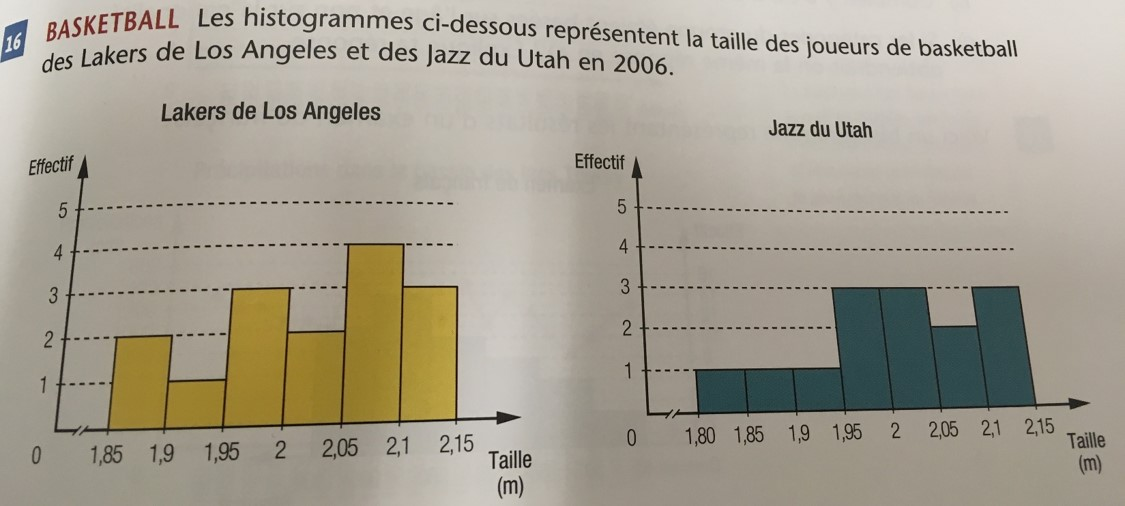
\includegraphics[scale=0.4]{Basket}
\end{center}

Quelle équipe a les plus grands joueurs?\\

\pause
\vspace{0.1in} La réponse n'est pas simple. On peut calculer et comparer les moyennes et/ou les médianes. Regarder l'étendue. Les valeurs des quartiles, .... 


%Vérifier si une moyenne est plus grande que l'autre, c'est maintenant le raisonnement mathématique. Comprendre l'intérêt de comparer les moyennes et savoir ce que ça veut dire pour la question, c'est plus une question statistique. 

%
%Deux niveaux de variabilité : 
%- Dans un ensemble de données, il y a une certaine variabilité. 
%- L'ensemble de données observé peut être considéré comme un ensemble aléatoire. 
%Soit si c'est tiré d'une population plus grande. 
%Soit si c'est parce que les valeurs observées elle-mêmes sont aléatoires. 


\end{frame}


\begin{frame}{Autre exemple - Dans quelle école les tailles sont-elles les plus variables?}


\begin{center}
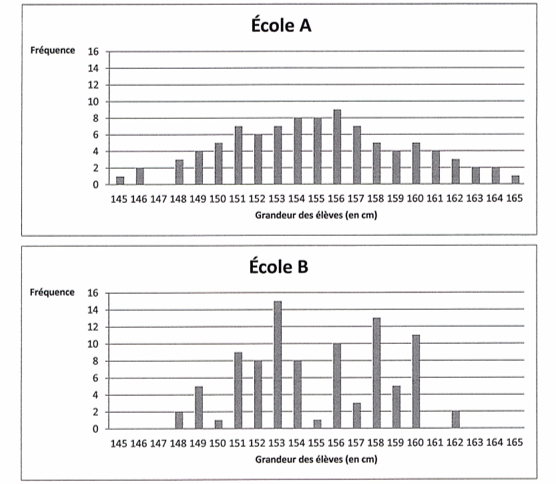
\includegraphics[scale=0.6]{Bandes_Ecoles}
\end{center}


\end{frame}


\begin{frame}{Matière du cours : Chapitre 2}



\begin{enumerate}
\item Plusieurs représentations numériques et graphiques. 
\item Comment les calculer / construire.
\item Comment les interpréter. 
\item Comment choisir celle qui est appropriée. 
\item Comment des statistiques différentes peuvent donner des visions différentes d'un même jeu de données.
\item L'impact d'une transformation linéaire des observations sur ces représentations.
\item L'impact de la sélection de l'échantillon sur la représentativité de ces mesures. 
\end{enumerate}


\end{frame}



\begin{frame}{Deuxième niveau de variabilité}

\begin{center}
{ \Large \alert{On considère les données observées elles-mêmes comme étant aléatoires. }}
\end{center}

\pause
\vspace{0.2in}
Cette variabilité peut provenir de deux sources :
\begin{enumerate}
\item Échantillonnage aléatoire d'une population finie
\item Données tirées d'un modèle statistique  \\
ex. $X_i \overset{iid}{\sim} N(0,\sigma^2), i = 1,\ldots, n$
\end{enumerate} 



\end{frame}


\begin{frame}{Inférence informelle}

\alert{On tient compte de l'aspect aléatoire des données pour généraliser à une population finie ou à un modèle. Nos conclusions seront alors plus nuancées. }

\pause

\vspace{0.1in}
{ Ex. Des moyennes échantillonnales différentes ne veulent pas nécessairement dire que les moyennes des populations sont différentes. }


\vspace{0.1in}

\pause

Note: Ce sont tout de même plus que des intuitions! Nos conclusions sont basées sur un certain raisonnement statistique.
%(Je ne suis donc pas complètement convaincue par la formulation du PFEQ.)

\pause
\vspace{0.2in}
On peut se rendre jusqu'ici dans un cours de secondaire. 

\end{frame}


\begin{frame}{Inférence formelle}

\alert{On teste formellement l'hypothèse d'intérêt à l'aide de la théorie statistique. }

\pause

\vspace{0.2in}
Le raisonnement statistique s'appuie ici sur la théorie des probabilités pour guider nos conclusions. On peut contrôler les probabilités d'erreur. 

\pause

\vspace{0.2in}
Les dérivations théoriques sont toutefois basées sur certains postulats/hypothèses. Pour que l'inférence soit valide, il faut que ceux-ci soient respectés.

\end{frame}

\begin{frame}{Matière du cours : Chapitres 3, 4 et 5}

{ \small 
\vspace*{-0.15in}
\begin{table}
\begin{tabular}{p{5cm}|p{5cm}}
Une variable continue & Inférence sur une moyenne \newline Inférence sur une variance \\[5pt]
\hline \\[1pt]
\pause
Une variable catégorique & Inférence sur une proportion \\[5pt]
\hline  \\[1pt]
\pause
Une variable continue et une variable catégorique (2 cat.) & Comparaison de moyennes \newline Comparaison de variances \\[5pt] 
\hline  \\[1pt]
\pause
Deux variables continues & Régression linéaire simple \\[5pt]
\hline \\[1pt]
\pause
Deux variables catégoriques & Test du khi-carré \newline Différence de proportions \newline (si 2 catégories par variable) 
\end{tabular}
\end{table}
}

\end{frame}


\begin{frame}{Matière du cours : Chapitre 1}

Avant toutes choses, il faut obtenir des données!

\begin{enumerate}
\item Différents modes de collecte de données
\item Comment faire un sondage ou une expérience de façon appropriée
\item Dans quelles circonstances peut-on généraliser / conclure à la causalité
\item Sources de biais à éviter
\end{enumerate}


\end{frame}

\end{document}



\begin{frame}{Estimation - principe}

\begin{center}
{\Large 
On souhaite un estimateur sans biais et avec la plus petite variance possible.
}
\end{center}

\end{frame}

\begin{frame}{Intervalle de confiance - principe}

Un \textbf{intervalle de confiance à $100(1-\alpha)\%$} pour $\theta$ est de la forme $[L,U]$, où $L$ et $U$ sont des statistiques telles que 
\begin{equation*}
P(L \leq \theta \leq U) = 1 - \alpha. \label{IC}
\end{equation*}
On crée un intervalle de confiance tel que si on tirait de la population ou du modèle un grand nombre d'échantillons, et qu'on utilisait chacun d'eux pour créer un intervalle de confiance $[L,U]$ pour $\theta$, alors  $100(1-\alpha)\%$ de ces intervalles renfermeraient le vrai paramètre $\theta$. 


\end{frame}


\begin{frame}{Test d'hypothèse - Principes}

\begin{itemize} \itemsep1em
\item On choisit une statistique de test pour laquelle on connait la distribution sous $H_0$. 
\pause
\item Si la valeur observée de la statistique avec nos données est peu probable sous $H_0$, on rejette $H_0$.
\pause
\begin{itemize}
\item Comparer la statistique observée au seuil critique, soit le quantile approprié de la distribution sous $H_0$. 
\pause
\item Ou comparer la probabilité de voir une statistique aussi extrême ou plus extrême sous $H_0$ (valeur-p) à la probabilité d'erreur de type I désirée ($\alpha$).
\end{itemize}
\end{itemize}

\end{frame}


\begin{frame}{Test d'hypothèse - Principes (suite)}


\textbf{Validité}\\
Un test sera valide si les hypothèses (postulats) sont vérifiés. 
Pour un test non valide, on n'aura pas nécessairement la probabilité d'erreur de type I $\alpha$ telle que prédit par la théorie.

\pause
\vspace{0.2in}
\textbf{Puissance}\\
Un test est puissant s'il nous permet de rejeter l'hypothèse nulle lorsque l'hypothèse alternative est vraie. 
\pause
\vspace{0.05in}
Puisqu'on ne contrôle pas directement la puissance, elle est parfois faible. C'est pourquoi si on ne rejette pas $H_0$ on ne conclura pas directement que $H_0$ est vraie. Il se peut simplement que la puissance soit trop faible pour pouvoir rejeter $H_0$. 
\end{frame}

\begin{frame}{RLS : particularités}

\begin{enumerate}[<+->] \itemsep1em
\item On a vu 3 méthodes d'estimation différentes. Il faut savoir les appliquer, et connaitre leurs avantages et inconvénients. 
\item En plus d'inférence sur les paramètres $\beta_0$ et $\beta_1$, on fait de l'inférence sur l'espérance de $Y$ pour une valeur de $x_0$, et sur la prévision d'une valeur spécifique de $Y$ pour un $x_0$. 
\item On peut tester l'utilité du modèle d'une deuxième façon, avec l'ANOVA. Il faut comprendre l'idée derrière l'ANOVA et savoir l'appliquer et l'interpréter, incluant le coefficient de détermination.
\item Il y a plus de postulats à vérifier pour que l'inférence soit valide. Il faut savoir comment les tester. 
\end{enumerate}

\end{frame}

\begin{frame}{RLS des MC: À garder en tête}

\begin{enumerate}[<+->]
\item On ne teste que la \alert{corrélation linéaire} entre les variables.
\item Il se peut que la relation linéaire entre les variables soit significative ($\beta_1 \ne 0$), mais que la variable explicative n'explique pas une grande proportion de la variabilité de la variable réponse (petit $R^2$).
\item La RLS n'est pas symétrique\\ (pas la même droite si on échange $x$ et $Y$).
\item On peut démontrer qu'il y a un phénomène de régression vers la moyenne. 
\item Des erreurs de mesures de la variable indépendante causent un biais d'atténuation sur la valeur de la pente.
\item Il peut être nécessaire de transformer les variables pour que le modèle soit valide. 
\end{enumerate}



\end{frame}

\begin{frame}{Importance des données utilisées}


Toute démarche statistique nécessite des données de qualité. 

\vspace{0.1in}
La façon avec laquelle les données ont été collectées a un impact sur 
\begin{itemize}
\item la généralisabilité des résultats
\item la possibilité de conclure à une relation de cause à effet
\item les méthodes statistiques à utiliser
\item la fiabilité des résultats
\end{itemize} 


\vspace{0.1in}
%Par exemple, si des données sont entachées d'une erreur de mesure; on sera prudent avec nos résultats même si le test formel rejette l'égalité des moyennes.

\end{frame}

